\documentclass{beamer}
\usetheme{Warsaw}
\usepackage{graphicx}
\usepackage{caption}
\usepackage{subcaption}
\usepackage{longtable}
\usepackage{listings}
\usepackage{color}
%% The amssymb package provides various useful mathematical symbols
\usepackage{amssymb}
%% The amsthm package provides extended theorem environments
\usepackage{amsthm} 
\usepackage{amsmath} 
\usepackage{tmadd,tmath}
\usepackage[mathcal]{euscript} 
\usepackage{color}
\usepackage{textcomp}
\usepackage{algorithm,algorithmic}
\definecolor{listinggray}{gray}{0.9}
\definecolor{lbcolor}{rgb}{0.9,0.9,0.9}
\lstset{
  backgroundcolor=\color{lbcolor},
  tabsize=4,
  rulecolor=,
  language=c++,
  basicstyle=\scriptsize,
  upquote=true,
  aboveskip={1.5\baselineskip},
  columns=fixed,
  showstringspaces=false,
  extendedchars=true,
  breaklines=true,
  prebreak =
  \raisebox{0ex}[0ex][0ex]{\ensuremath{\hookleftarrow}},
  frame=single,
  showtabs=false,
  showspaces=false,
  showstringspaces=false,
  identifierstyle=\ttfamily,
  keywordstyle=\color[rgb]{0,0,1},
  commentstyle=\color[rgb]{0.133,0.545,0.133},
  stringstyle=\color[rgb]{0.627,0.126,0.941},
}

%% colors
\setbeamercolor{boxheadcolor}{fg=white,bg=black}
\setbeamercolor{boxbodycolor}{fg=black,bg=white}

%% slide numbers

%%---------------------------------------------------------------------------%%
\author{Stuart Slattery}

\date{\today} 
\title[Multilevel Monte Carlo Solvers for Linear Systems \hspace{1mm}
  \insertframenumber/\inserttotalframenumber]{Multilevel Monte Carlo
  Solvers for Linear Systems}
\begin{document}
\maketitle

%%---------------------------------------------------------------------------%%
\begin{frame}{Hardware-Based Motivation}

  \begin{itemize}
  \item Modern hardware is moving in two directions (Kogge,2011):
    \begin{itemize}
    \item Lightweight machines
    \item Heterogeneous machines
    \item Both characterized by low power and high concurrency
    \end{itemize}
    \medskip \medskip
  \item Some issues:
    \begin{itemize}
    \item Higher potential for both soft and hard failures (DOE,2012)
    \item Memory restrictions are expected with a continued decrease
      in memory/FLOPS
    \end{itemize}
    \medskip \medskip
  \item Potential resolution from Monte Carlo:
    \begin{itemize}
    \item Soft failures buried within the tally variance
    \item Hard failures mitigated by replication
    \item Memory savings over conventional methods
    \end{itemize}
  \end{itemize}

\end{frame}

%%---------------------------------------------------------------------------%%
\begin{frame}{Monte Carlo Methods for Discrete Linear Systems}

  \begin{itemize}
  \item First proposed by J. Von Neumann and S.M. Ulam in the 1940's
    \medskip \medskip
  \item Earliest published reference in 1950
    \medskip \medskip
  \item General lack of published work
    \medskip \medskip
  \item Modern work by Evans and others has yielded new
    applications\let\thefootnote\relax\footnote{\tiny{Thomas Evans and
        Scott Mosher, "A Monte Carlo Synthetic Acceleration method for
        the non-linear, time-dependent diffusion equation", American
        Nuclear Society - International Conference on Mathematics,
        Computational Methods and Reactor Physics, 2009.}}
  \end{itemize}

\end{frame}

%%---------------------------------------------------------------------------%%
\begin{frame}{Monte Carlo Linear Solver Preliminaries}

  \begin{itemize}
  \item Split the linear operator
  \end{itemize}

  \[
  \ve{A}\ve{x} = \ve{b} \ \ \ \rightarrow \ \ \ \ve{x} = \ve{H} \ve{x}
  + \ve{b}
  \]

  \[
  \ve{H} = \ve{I} - \ve{A}
  \]

  \medskip
  \begin{itemize}
  \item Generate the \textit{Neumann series}
  \end{itemize}
  
  \[
  \ve{A}^{-1} = (\ve{I}-\ve{H})^{-1} = \sum_{k=0}^{\infty} \ve{H}^k
  \]

  \medskip
  \begin{itemize}
  \item Require $\rho(\ve{H}) < 1$ for convergence
  \end{itemize}

  \[
  \ve{A}^{-1}\ve{b} = \sum_{k=0}^{\infty} \ve{H}^k\ve{b} = \ve{x}
  \]

\end{frame}

%%---------------------------------------------------------------------------%%
\begin{frame}{Monte Carlo Linear Solver Preliminaries}

  \begin{itemize}
  \item Expand the Neumann series
  \end{itemize}

  \[
  x_i = \sum_{k=0}^{\infty}\sum_{i_1}^{N}\sum_{i_2}^{N}\ldots
  \sum_{i_k}^{N}h_{i,i_1}h_{i_1,i_2}\ldots h_{i_{k-1},i_k}b_{i_k}
  \]

  \begin{itemize}
  \item Define a sequence of state transitions
  \end{itemize}
  
  \[
  \nu = i \rightarrow i_1 \rightarrow \cdots \rightarrow i_{k-1}
  \rightarrow i_{k}
  \]

  \begin{itemize}
  \item Use the adjoint Neumann-Ulam
    decomposition\let\thefootnote\relax\footnote{The Hadamard product
      $\ve{A} = \ve{B} \circ \ve{C}$ is defined element-wise as
      $a_{ij} = b_{ij} c_{ij}$.}
  \end{itemize}

  \[
  \ve{H}^{T} = \ve{P} \circ \ve{W}
  \]

  \[
  p_{ij} = \frac{|h_{ji}|}{\sum_j |h_{ji}|},\ w_{ij} =
  \frac{h_{ji}}{p_{ij}}
  \]

\end{frame}

%%---------------------------------------------------------------------------%%
\begin{frame}{Evolution of a Solution}

  \begin{figure}[htpb!]
    \begin{center}
      \scalebox{1.0}{ \input{heat_eq_setup.pdftex_t} }
    \end{center}
    \caption{\textbf{Poisson Problem.}
      \textit{Distributed source of 1.0 in the domain.}}
  \end{figure}

\end{frame}

%%---------------------------------------------------------------------------%%
\begin{frame}{Evolution of a Solution}

  \begin{figure}[h!]
    \begin{center}
      \includegraphics<1>[width=4in]{adjoint_1.png}
      \includegraphics<2>[width=4in]{adjoint_10.png}
      \includegraphics<3>[width=4in]{adjoint_100.png}
      \includegraphics<4>[width=4in]{adjoint_1000.png}
      \includegraphics<5>[width=4in]{adjoint_10000.png}
      \includegraphics<6>[width=4in]{adjoint_100000.png}
      \includegraphics<7>[width=4in]{adjoint_1000000.png}
      \includegraphics<8>[width=4in]{adjoint_10000000.png}
    \end{center}
    \caption{
      \only<1>{\textbf{Adjoint solution to Poisson Equation.}
        \textit{\sn{1}{0} total histories, 0.286 seconds CPU time.} }
      \only<2>{\textbf{Adjoint solution to Poisson Equation.}
        \textit{\sn{1}{1} total histories, 0.278 seconds CPU time.} }
      \only<3>{\textbf{Adjoint solution to Poisson Equation.}
        \textit{\sn{1}{2} total histories, 0.275 seconds CPU time.} }
      \only<4>{\textbf{Adjoint solution to Poisson Equation.}
        \textit{\sn{1}{3} total histories, 0.291 seconds CPU time.} }
      \only<5>{\textbf{Adjoint solution to Poisson Equation.}
        \textit{\sn{1}{4} total histories, 0.428 seconds CPU time.} }
      \only<6>{\textbf{Adjoint solution to Poisson Equation.}
        \textit{\sn{1}{5} total histories, 1.76 seconds CPU time.} }
      \only<7>{\textbf{Adjoint solution to Poisson Equation.}
        \textit{\sn{1}{6} total histories, 15.1 seconds CPU time.} }
      \only<8>{\textbf{Adjoint solution to Poisson Equation.}
        \textit{\sn{1}{7} total histories, 149 seconds CPU time.} } 
    }
  \end{figure}

\end{frame}

%%---------------------------------------------------------------------------%%
\begin{frame}{Model Problem}

  Choose a simple homogeneous problem with Dirichlet conditions:
  \[
  \nabla^2 x = 0, \ \ve{x}_1 = 0,\ \ \ve{x}_N = 0
  \]

  Second order finite difference:
  \[
  (\nabla \ve{u})_i = \frac{\ve{u}_{i-1} - 2 \ve{u}_{i} + \ve{u}_{i+1}}{h^2}
  \]

  Monte Carlo requires $\rho(\ve{H})$ so we scale by the diagonal:
  \[
  \ve{M}^{-1}\ve{A}\ve{x} = \ve{0}
  \]

  Choose initial guess to be some Fourier mode
  \[
  \ve{x}^0_i = \sin\Bigg( \frac{ik\pi}{N} \Bigg)
  \]

\end{frame}

%%---------------------------------------------------------------------------%%
\begin{frame}{Error Analysis}

  \begin{columns}

    \begin{column}{0.5\textwidth}
      \begin{figure}[h!]
        \begin{center}
          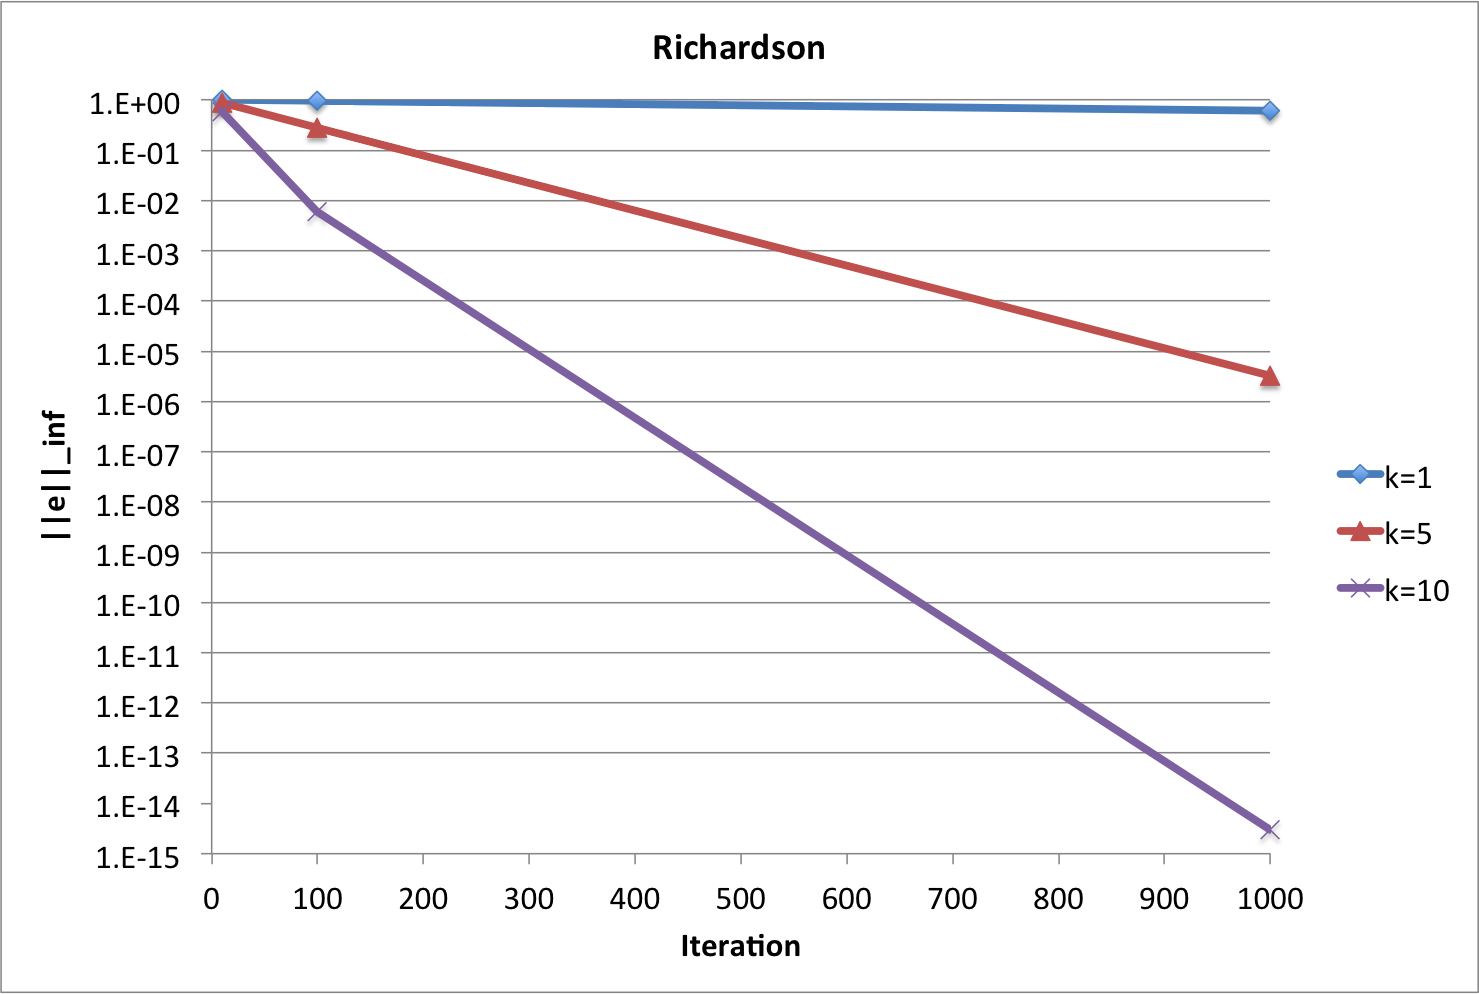
\includegraphics[width=2in]{richardson.png}
        \end{center}
        \caption{\textbf{Convergence of Richardson's iteration.}
          \textit{Better for larger wave numbers.}}
        \label{fig:richardson}
      \end{figure}
    \end{column}

    \begin{column}{0.5\textwidth}
      \begin{figure}[h!]
        \begin{center}
          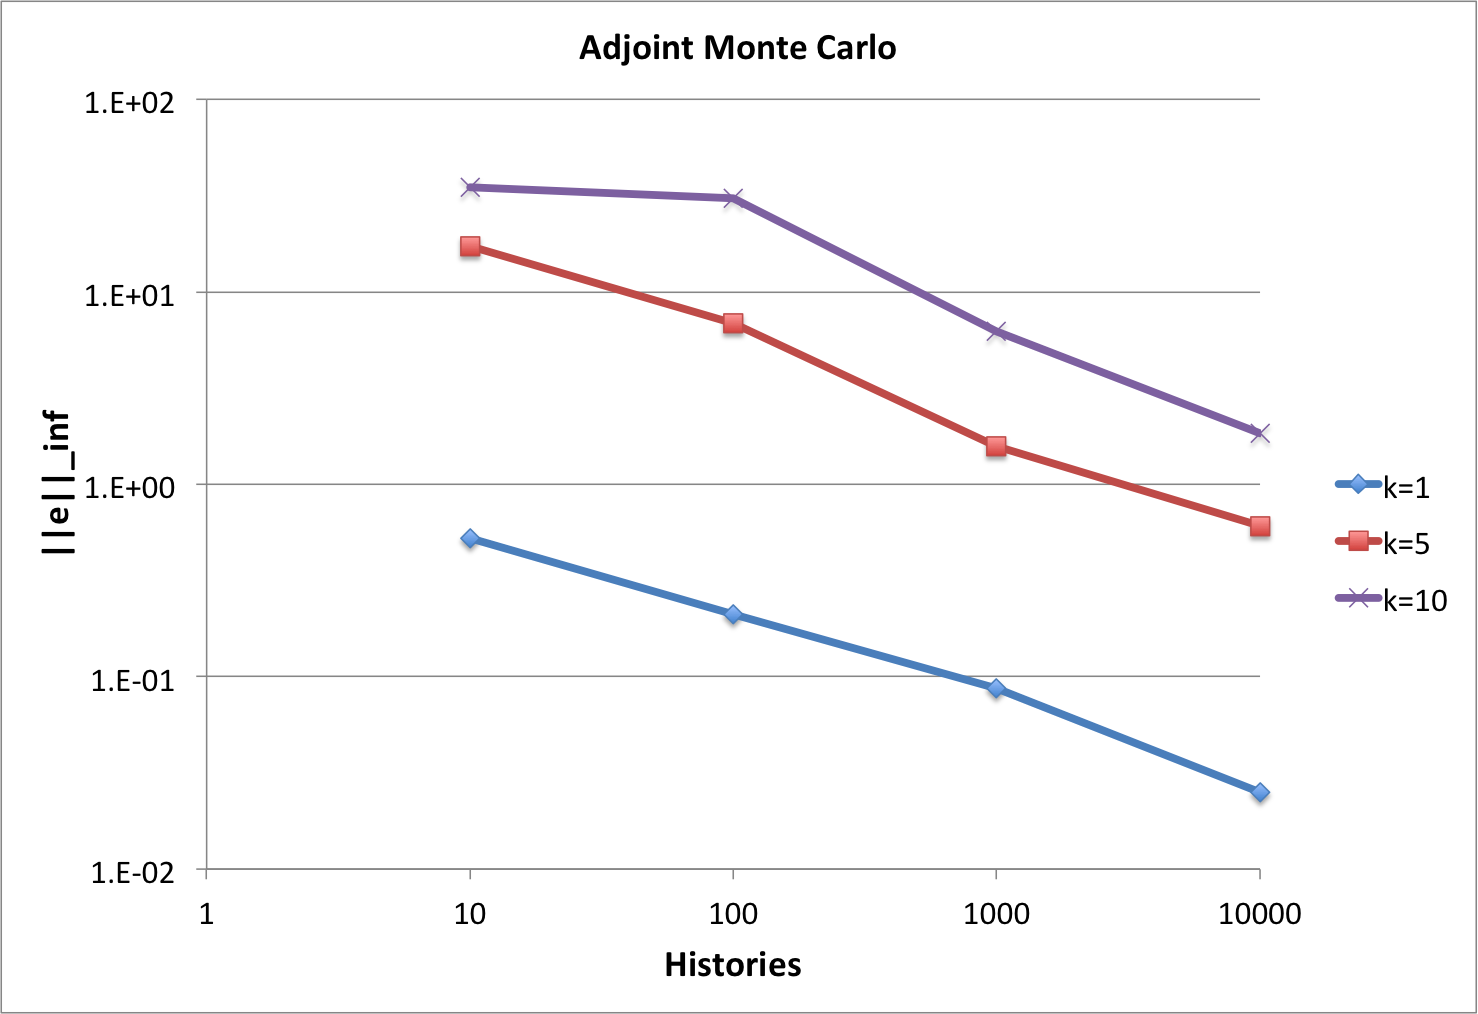
\includegraphics[width=2in]{adjoint_mc.png}
        \end{center}
        \caption{\textbf{Convergence of the adjoint Monte Carlo
            method.} \textit{Better for smaller wave numbers.} }
        \label{fig:adjoint_mc}
      \end{figure}
    \end{column}

  \end{columns}

\end{frame}

%%---------------------------------------------------------------------------%%
\begin{frame}{Error Analysis}

  \begin{columns}

    \begin{column}{0.5\textwidth}

      \begin{figure}[h!]
        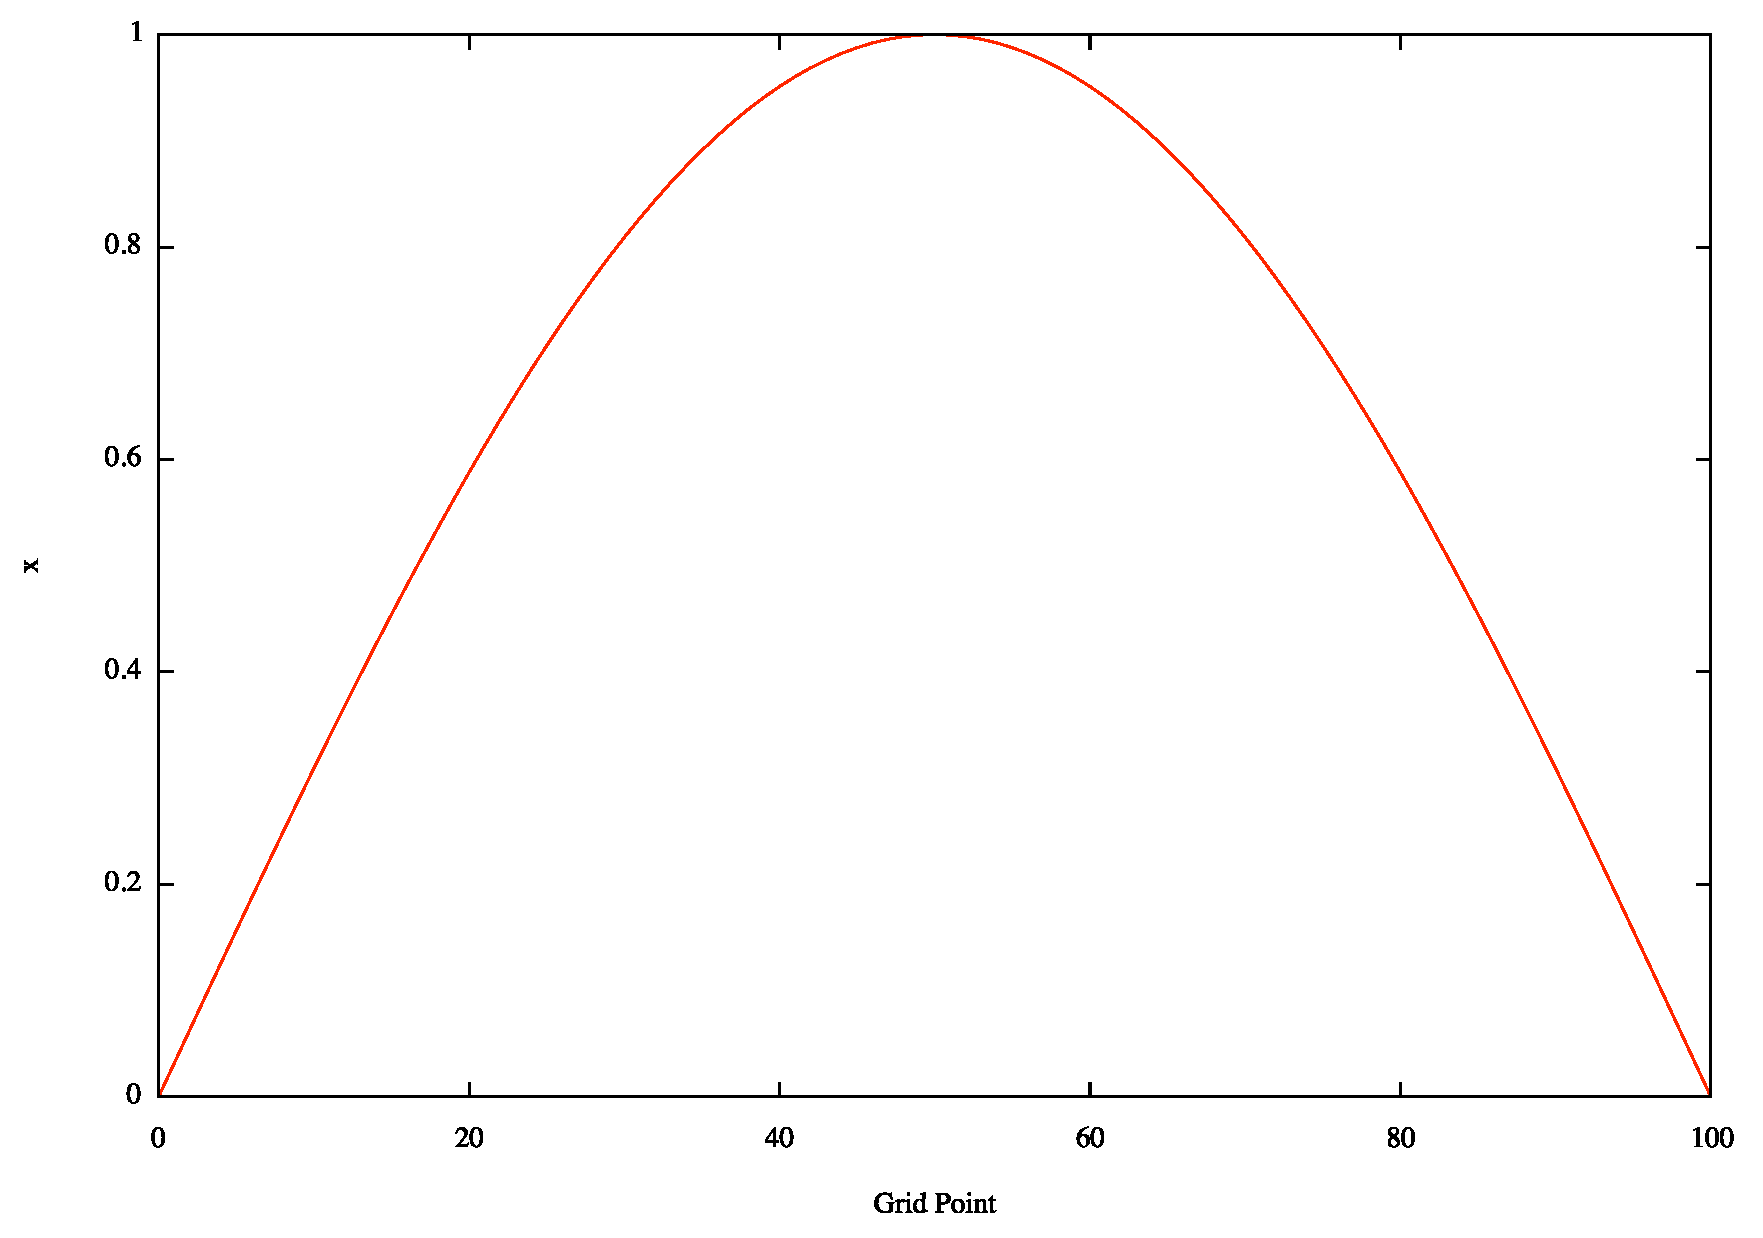
\includegraphics[width=1.5in]{mode_1.pdf}
        \caption{\textbf{$k = 1$.}}
      \end{figure}

      \begin{figure}[b]
        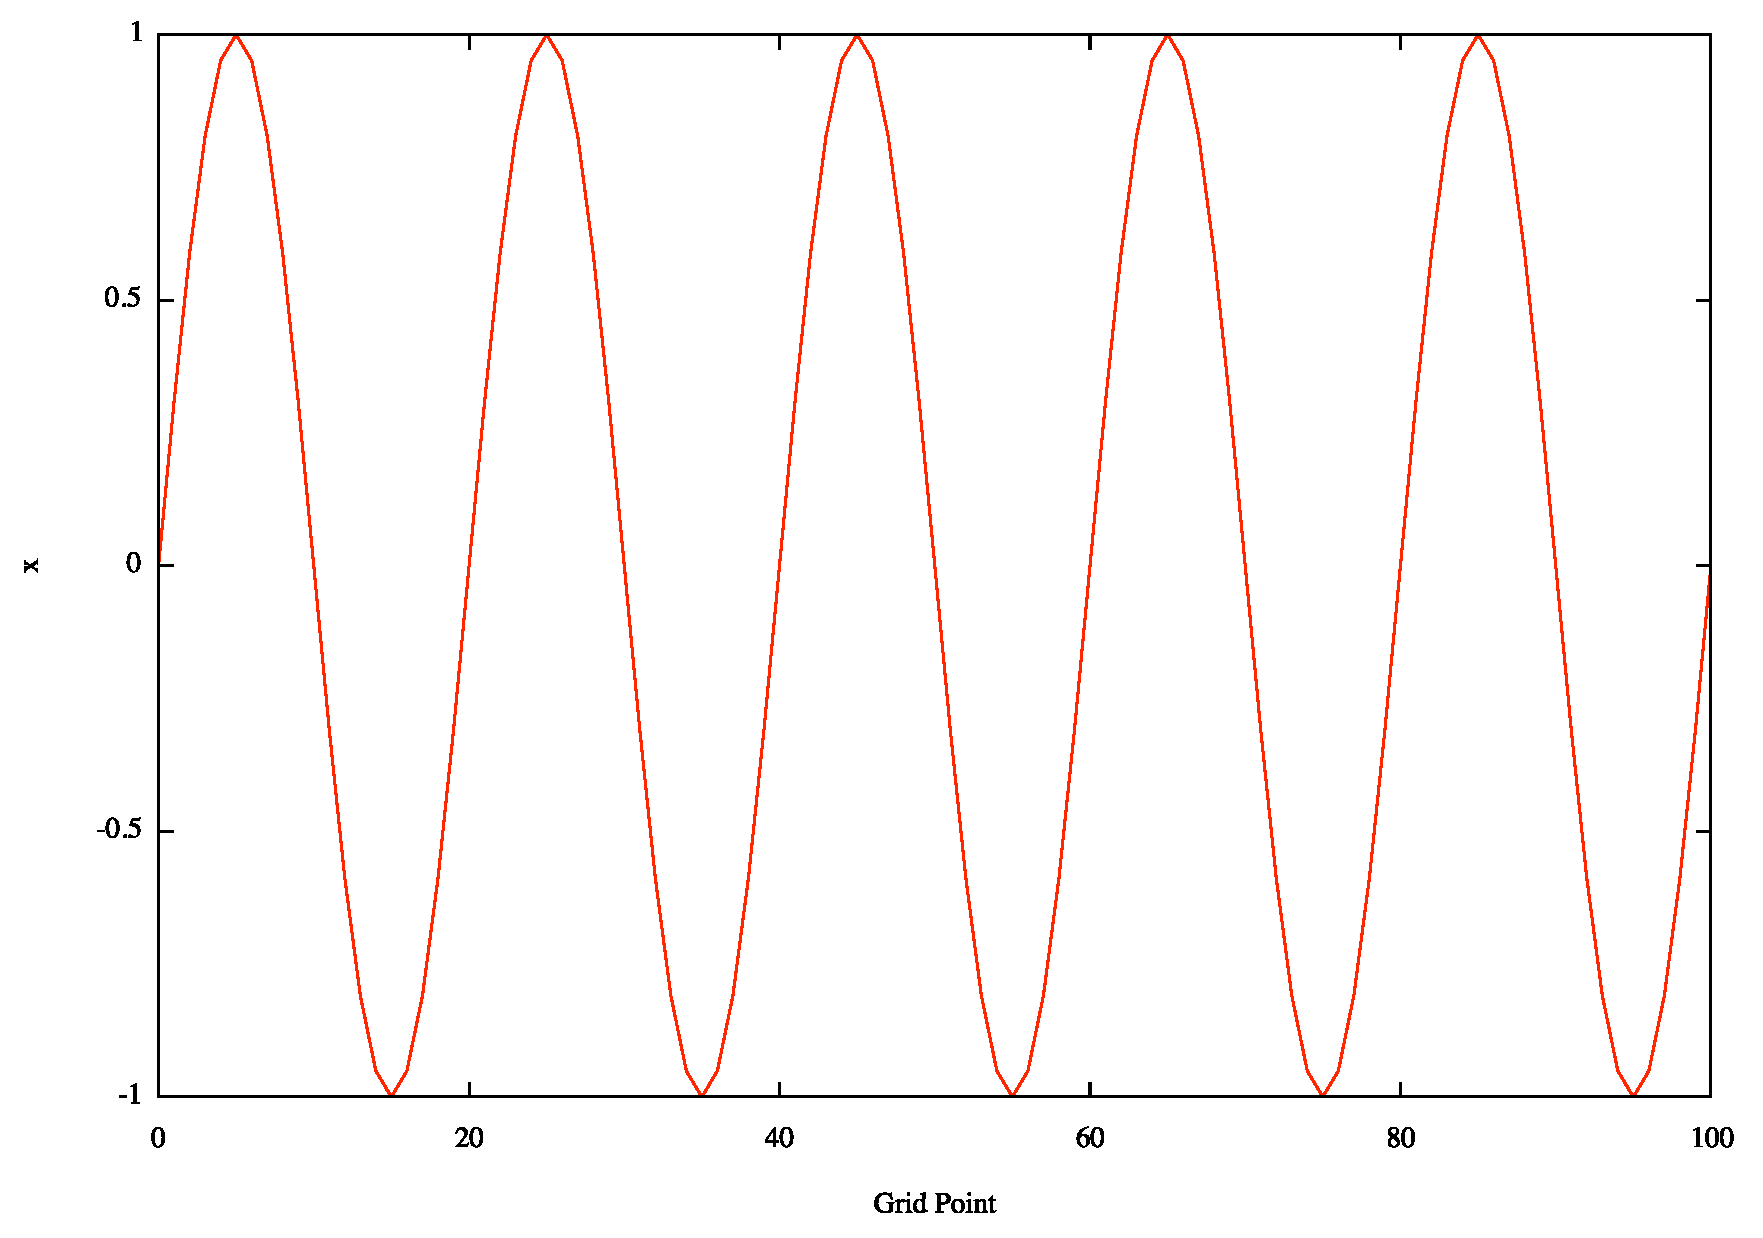
\includegraphics[width=1.5in]{mode_10.pdf}
        \caption{\textbf{$k = 10$.}}
      \end{figure}

    \end{column}

    \begin{column}{0.5\textwidth}

      { \tiny
      \begin{table}[h!]
        \begin{center}
          \begin{tabular}{cc}\hline\hline
            \multicolumn{1}{c}{\textbf{Wave Number}} & 
            \multicolumn{1}{c}{\textbf{Time per History (s)}} \\
            \hline
            1 & 1 \\
            5 & 0.85 \\
            10 & 0.83 \\
            \hline\hline
          \end{tabular}
        \end{center}
        \caption{\textbf{Normalized average CPU time per history.}}
        \label{tab:mc_timing}
      \end{table}
      }

      \begin{itemize}
        \item $\sigma(A)$ dictates the characteristics of the Markov
          chain
        \item $N$ dictates the convergence of the Monte Carlo
      \end{itemize}

    \end{column}

  \end{columns}

\end{frame}

%%---------------------------------------------------------------------------%%
\begin{frame}{Multilevel Monte Carlo Methods}

  \begin{itemize}
  \item Formalized by Heinrich for integral equations in 2001 and by
    Giles in 2008 for finance calculations
  \item Recent work includes Bayesian inference techniques for
    stochastic PDEs in ground water flow
  \end{itemize}

\end{frame}

%%---------------------------------------------------------------------------%%
\begin{frame}{Multilevel Expectation}

  We start first with the standard Monte Carlo estimator for the
  solution vector:
  \[
  \hat{\ve{x}} = \frac{1}{N} \sum_{m=1}^N x^m
  \]

  \medskip

  Consider $L$ levels with level 0 the finest $L$ the coarsest:
  \[
  E(\ve{x}_{0}) = E(\ve{x}_{L}) + E(\ve{x}_{L-1} - \ve{x}_{L}) +
  E(\ve{x}_{L-2} - \ve{x}_{L-1}) + \dots + E(\ve{x}_{0} - \ve{x}_{1})
  \]

  \medskip

  Reduce to a sum:
  \[
    \hat{\ve{y}}_{l} = \frac{1}{N_l} \sum_{m=1}^{N_l} (x^m_{l} -
    x^m_{l+1})
  \]

\end{frame}

%%---------------------------------------------------------------------------%%
\begin{frame}{Multilevel Expectation}

  Build a correction estimator for a given level $l$:
  \[
    \hat{\ve{y}}_{l} = \frac{1}{N_l} \sum_{m=1}^{N_l} (x^m_{l} -
    x^m_{l+1})
  \]

  \medskip

  Leaving a final multilevel estimator of:
  \[
  \hat{\ve{x}} = \sum_{l=0}^L \hat{\ve{y}}_{l}
  \]

  \medskip

  \textbf{Critical observation:} $x^m_{l}$ and $x^m_{l+1}$
  must be constructed from the \textit{same} Markov chain

\end{frame}

%%---------------------------------------------------------------------------%%
\begin{frame}{Constructing Multilevel Estimates}

  Number of samples at each level should be determined from the
  estimated variance. For simplicity:
  \[
  N_l = M^{-3(L-l)/2}N
  \]

  \medskip

  Define a \textit{prolongation operator}, $\ve{P}_l$, which maps a
  vector defined on grid $l+1$ to a vector defined on grid $l$ and a
  \textit{restriction operator}, $\ve{R}_l$, which maps a vector
  defined on grid $l$ to a vector defined on grid $l+1$
  \[
  E(\ve{x}_{l} - \ve{x}_{l+1}) = \Big(\ve{I} - \ve{P}_l \ve{R}_l\Big)
  \hat{\ve{x}}_{l}
  \]

\end{frame}

%%---------------------------------------------------------------------------%%
\begin{frame}[fragile]{Multilevel Monte Carlo Solver}

  \begin{algorithm}[H]
    \caption{\small Multilevel Monte Carlo Method}
    \label{alg:mlamc}
    \begin{algorithmic}[1]
      { \small
      \FOR{ l = 0...L }
      \STATE  $\ve{P}_l = P(\ve{A}_l)$
      \COMMENT{Build the prolongation and restriction operators for
        the $l^{th}$ level.}
      \STATE $\ve{R}_l = c \ve{P}_l^T$
      \STATE $\ve{r}_l = \ve{b}_l - \ve{A}_l \ve{x}_l^0$
      \COMMENT{Build the $l^{th}$ level residual.}
      \STATE $\ve{d}_l = \hat{\ve{A}}_l^{-1} \ve{r}_l$
      \COMMENT{Solve the $l^{th}$ level problem with adjoint Monte
        Carlo}
      \IF{ l != L }
      \STATE $\ve{d}_l = (\ve{I} - \ve{P}_l\ve{R}_l) \ve{d}_{l}$
      \COMMENT{Apply the multilevel tally}
      \STATE $\ve{A}_{l+1} = \ve{R}_l \ve{A}_l \ve{P}_l$
      \COMMENT{Construct the next level.}
      \STATE $\ve{x}_{l+1}^0 = \ve{R}_l \ve{x}_l^0$
      \STATE $\ve{b}_{l+1} = \ve{R}_l \ve{b}_l$
      \ENDIF
      \ENDFOR

      \FOR{ l = L...1 }
      \STATE $\ve{d}_{l-1} = ( \ve{I} + \ve{P}_{l} ) \ve{d}_{l}$
      \COMMENT{Collapse the tallies to the finest grid}
      \ENDFOR
      \STATE $\ve{x} = \ve{x}^0 + \ve{d}_0$
      }
    \end{algorithmic}
  \end{algorithm}

\end{frame}

%%---------------------------------------------------------------------------%%
\begin{frame}{Numerical Experiments}

\end{frame}

%%---------------------------------------------------------------------------%%
\begin{frame}{Geometric Multigrid Example}

\end{frame}

%%---------------------------------------------------------------------------%%
\begin{frame}{Geometric Multigrid Example}

\end{frame}

%%---------------------------------------------------------------------------%%
\begin{frame}{Algebraic Multigrid Example}

\end{frame}

%%---------------------------------------------------------------------------%%
\begin{frame}{Algebraic Multigrid Example}

\end{frame}

%%---------------------------------------------------------------------------%%
\begin{frame}{Summary}

\end{frame}

%%---------------------------------------------------------------------------%%

\end{document}
